% ==========================================================================
% CHAPTER 2 -- METHODOLOGY
%
% Describes how the work was done, in enough detail that another EEE student
% could repeat it and obtain the same result.
% ==========================================================================

\chapter{Methodology}
\label{ch:methodology}

This chapter describes the complete experimental pipeline of the thesis: the
public databases used, the beat-extraction and preprocessing stages, the
record-disjoint partitioning scheme, the auxiliary feature vector, the two
network architectures (the CNN--BiLSTM--attention hybrid and MSFT-Net), the
training and imbalance-handling procedures, and the statistical evaluation,
explainability, and deployment methods.


\section{Introduction}
\label{sec:ch2_intro}

The aim of this chapter is to present the design of the study in a way that
allows exact reproduction. Section~\ref{sec:design} states the overall
research design; Section~\ref{sec:materials} describes the databases and
computing tools; Section~\ref{sec:data_analysis} describes signal
preprocessing, beat extraction, and the auxiliary features;
Section~\ref{sec:math} gives the mathematical formulation of the network
architectures; Section~\ref{sec:proposed_methodology} details the proposed
pipeline; Section~\ref{sec:workflow} describes the training workflow and
imbalance handling; and Section~\ref{sec:eval_criteria} defines the
performance evaluation criteria and statistical procedures.


\section{Research Design}
\label{sec:design}

The work is a retrospective computational study: pre-recorded, publicly
available, and de-identified ECG data are used to develop and test beat
classifiers. The main analysis is a supervised five-class classification
problem (N, S, V, F, Q) solved with two deep learning architectures, with a
secondary six-category ECG experiment used to quantify the effect of the
evaluation protocol. A record-disjoint, inter-patient partitioning scheme is
the central design constraint: no patient contributes beats to more than one
partition, so that the reported performance measures genuine generalisation
to unseen patients. Secondary design constraints are (i) class-balancing
operations are applied to the training partition only, (ii) all auxiliary
statistics are computed from training beats only, and (iii) the final model
must fit within the flash, RAM, and latency budgets of a
microcontroller-class wearable device.


\section{Materials \& Equipment}
\label{sec:materials}

\subsection{Databases}

The primary data source is the MIT-BIH Arrhythmia Database, which comprises
48 half-hour, two-channel ambulatory electrocardiograms sampled at 360~Hz
with beat annotations \cite{moody2001mitbih,goldberger2000physionet}. Two
auxiliary databases extend the corpus: the MIT-BIH Normal Sinus Rhythm
Database (18 recordings, used to augment the normal class) and the BIDMC
Congestive Heart Failure Database (15 recordings of about 20 hours each,
sampled at 250~Hz) \cite{goldberger2000physionet,baim1986chf}. Beat-level
labels originate only from the MIT-BIH Arrhythmia annotations, which are
grouped into the five ANSI/AAMI EC57 classes. The NSR recordings carry no
beat annotations and are folded into the normal class; the CHF recordings
likewise carry no beat annotations and are labelled purely by database
provenance as a separate CHF-derived clinical-condition category in the
secondary experiment. CHF is a cardiovascular condition rather than an
AAMI beat class, so the secondary task is a six-category ECG problem, not a
six-class arrhythmia problem. All data are
de-identified and publicly available through PhysioNet, so no ethical
approval was required for this retrospective study.

\subsection{Software and hardware tools}

The models were implemented in Python 3 using TensorFlow (with Keras),
NumPy, and scikit-learn for metric computation. Training was performed on a
GPU-equipped workstation. Deployment measurements were carried out on an
STM32 microcontroller (128\,KB RAM, 512\,KB flash) using the TensorFlow Lite
Micro runtime. Random seeds in Python, NumPy, and TensorFlow were set to 42
for reproducibility.


\section{Data Analysis Techniques}
\label{sec:data_analysis}

\subsection{Signal preprocessing and beat extraction}

Each ECG signal was filtered with a second-order Butterworth band-pass
filter (cut-off frequencies 0.5 and 40~Hz) applied as a zero-phase filter.
For the MIT-BIH Arrhythmia Database, the reference beat annotations were
used; where no beat label was provided, R-wave peaks were detected with the
Pan--Tompkins algorithm \cite{pan1985qrs}, which combines differentiation,
squaring, moving-window integration, and adaptive thresholding.
Signals sampled at frequencies other than 360~Hz were linearly resampled to
360~Hz. For each detected R-peak, a one-second window (360 samples) centred
on the peak was extracted; windows extending beyond the recording boundary
were omitted, and the MLII lead was used whenever available. Scaling
parameters for each retained waveform were estimated using only the
training partition. The possible impact of sampling and bandwidth
differences across sources was tested separately by resampling all beats to
a common 128~Hz.

\subsection{Auxiliary feature extraction}

Four signal windows of raw waveform were used together with an auxiliary
feature vector of 107 dimensions. Rhythm features included pre- and
post-RR intervals and their ratio, RR intervals normalised relative to
rolling local and record-level medians, the local RR coefficient of
variation, and indices of prematurity and compensatory pause. These
quantities were computed from the entire R-peak sequence before beat
filtering, then indexed to the retained beats. Morphological features were
computed over the interval 250--80~ms prior to the R-peak, including P-wave
morphology and QRS duration and shape features, and were compared against
high-quality normal-beat templates from the same record as well as global
normal and ventricular templates. Only raw training beats were used to
construct the global templates and the synthetic normal-to-ventricular
fusion continuum. The auxiliary features were scaled using training-partition
statistics (median and interquartile range).


\section{Mathematical Formulation}
\label{sec:math}

\subsection{CNN--BiLSTM--attention hybrid}

The hybrid model, whose block diagram is shown in
Figure~\ref{fig:hybrid_arch}, processes the waveform with three cascaded
1-D CNN blocks
with 64, 128, and 256 filters, each followed by batch normalisation, ReLU
activation, and max pooling. The sequence output of the final convolutional
stage is passed to a bidirectional LSTM with 128 units per direction, and
the LSTM output is pooled with additive temporal attention:

% ----- Figure: intra-patient hybrid model architecture -------------------
% Manual compliance: caption below the figure and centred (Instruction 14a),
% float placed at the top of a page ([!t]), never directly under a
% subtitle (Instruction 14f). The \IfFileExists guard keeps the book
% compilable while the diagram file is not yet present.
\begin{figure}[!t]
\centering
\IfFileExists{figures/System_Architecture/hybrid_cnn_bilstm_attention.png}{%
  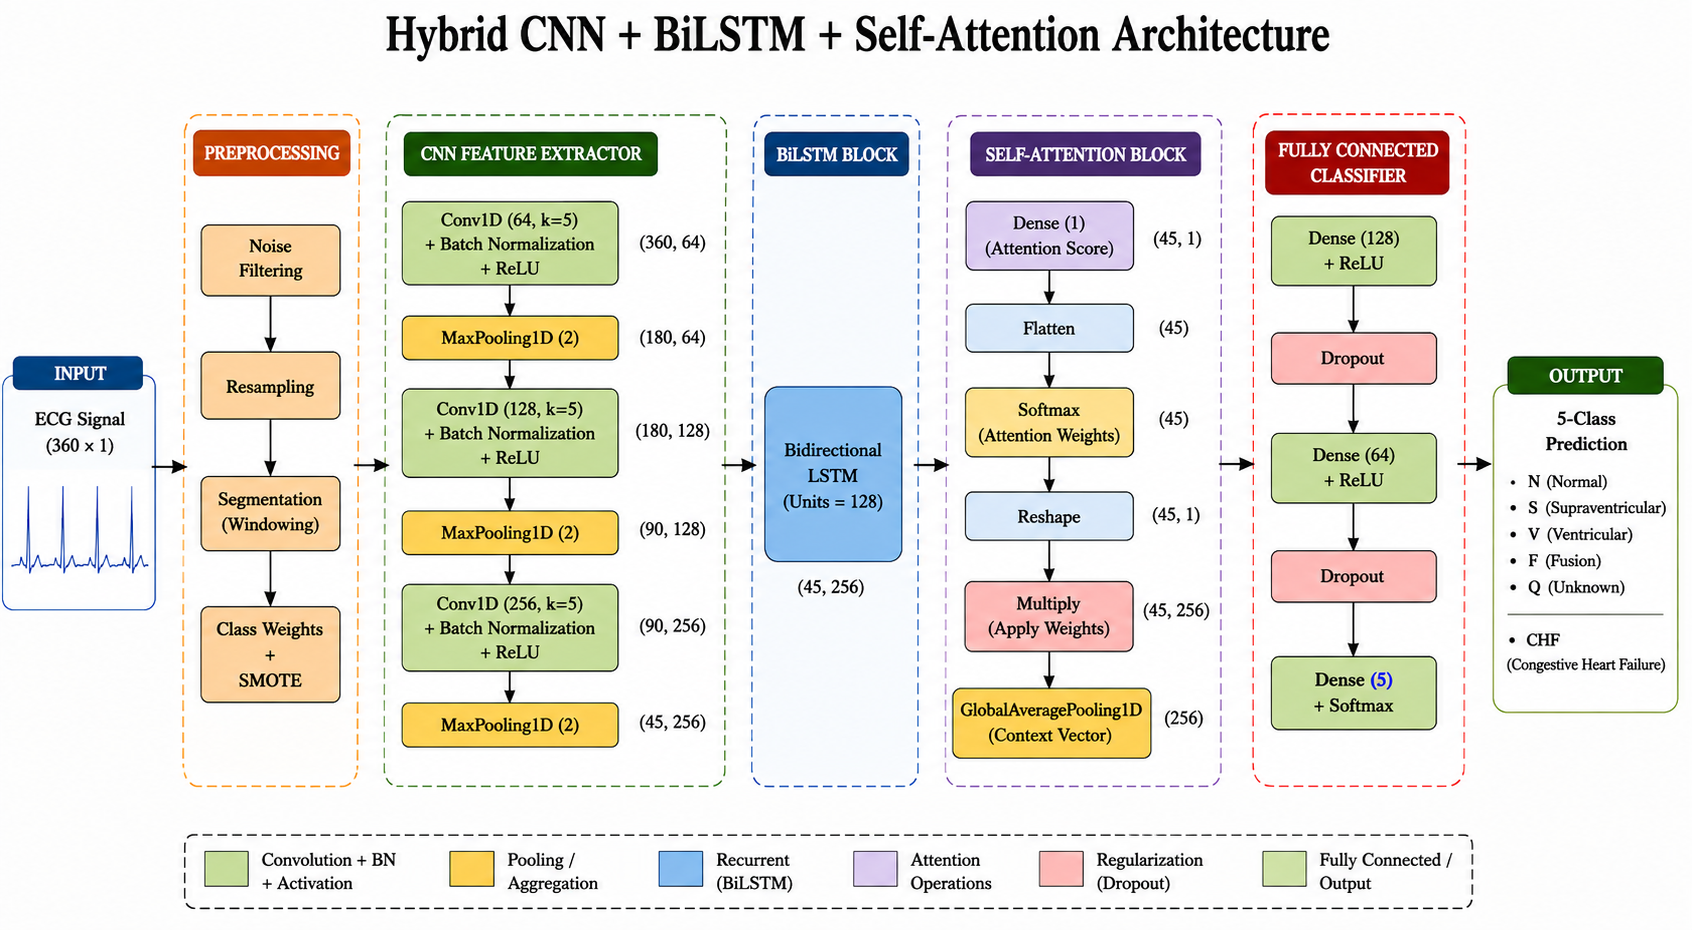
\includegraphics[width=0.95\linewidth]{figures/System_Architecture/hybrid_cnn_bilstm_attention.png}%
}{%
  \fbox{\parbox[c][2.6in][c]{0.92\linewidth}{\centering\footnotesize
    ADD THE HYBRID MODEL BLOCK DIAGRAM\\[4pt]
    \texttt{figures/System\_Architecture/}\\
    \texttt{hybrid\_cnn\_bilstm\_attention.png}}}%
}
\caption{Block diagram of the intra-patient CNN--BiLSTM--attention hybrid architecture}
\label{fig:hybrid_arch}
\end{figure}

\begin{equation}
  \alpha_{t} = \frac{\exp\left(\mathbf{v}^{\top}\tanh(\mathbf{W}\mathbf{h}_{t})\right)}{\sum_{t'}\exp\left(\mathbf{v}^{\top}\tanh(\mathbf{W}\mathbf{h}_{t'})\right)}
  \label{eq:attention}
\end{equation}

where $\mathbf{h}_{t}$ is the hidden state at time step $t$, and
$\mathbf{W}$ and $\mathbf{v}$ are learnable attention parameters. The
pooled waveform representation $\sum_{t}\alpha_{t}\mathbf{h}_{t}$ is
combined with a 48-unit dense branch that processes the auxiliary feature
vector, and the concatenation feeds the dense softmax classifier.

\subsection{MSFT-Net}

The comparison model, MSFT-Net, begins with three parallel
depthwise-separable convolutional blocks with kernel sizes 5, 11, and 21
samples followed by a single pointwise fusion layer. Three residual,
depthwise-separable stages follow, each including squeeze-and-excitation
(SE) channel gating and feature-wise linear modulation (FiLM) conditioned on
the auxiliary vector. SE gating reweights the channels of a feature map:

\begin{equation}
  \mathbf{x}' = \sigma\left(\mathbf{W}_{2}\,\mathrm{ReLU}(\mathbf{W}_{1}\,\mathrm{GAP}(\mathbf{x}))\right) \odot \mathbf{x}
  \label{eq:se}
\end{equation}

where GAP is global average pooling, $\sigma$ is the sigmoid function, and
$\odot$ is the Hadamard product. FiLM applies per-channel affine
conditioning derived from the auxiliary vector:

\begin{equation}
  \mathbf{y} = \boldsymbol{\gamma}(\mathbf{a}) \odot \mathbf{x} + \boldsymbol{\beta}(\mathbf{a})
  \label{eq:film}
\end{equation}

where $\boldsymbol{\gamma}$ and $\boldsymbol{\beta}$ are generated by dense
layers from the auxiliary vector $\mathbf{a}$. The overall data flow of
MSFT-Net -- the inter-patient deployment model -- is summarised in
Figure~\ref{fig:msft_arch}. The same late
auxiliary-feature fusion, global average pooling, and classification head
are used as in the hybrid. Two additional CNN-only and CNN--BiLSTM models
without attention were trained as ablation baselines, and the
microcontroller implementation used a separate single-input CNN.

% ----- Figure: inter-patient MSFT-Net architecture ------------------------
\begin{figure}[!t]
\centering
\IfFileExists{figures/System_Architecture/msft_net_architecture.png}{%
  % Portrait diagram (853x1280): sized below full text width to preserve
  % quality (>=200 dpi) and keep figure + caption on one page at natural ratio.
  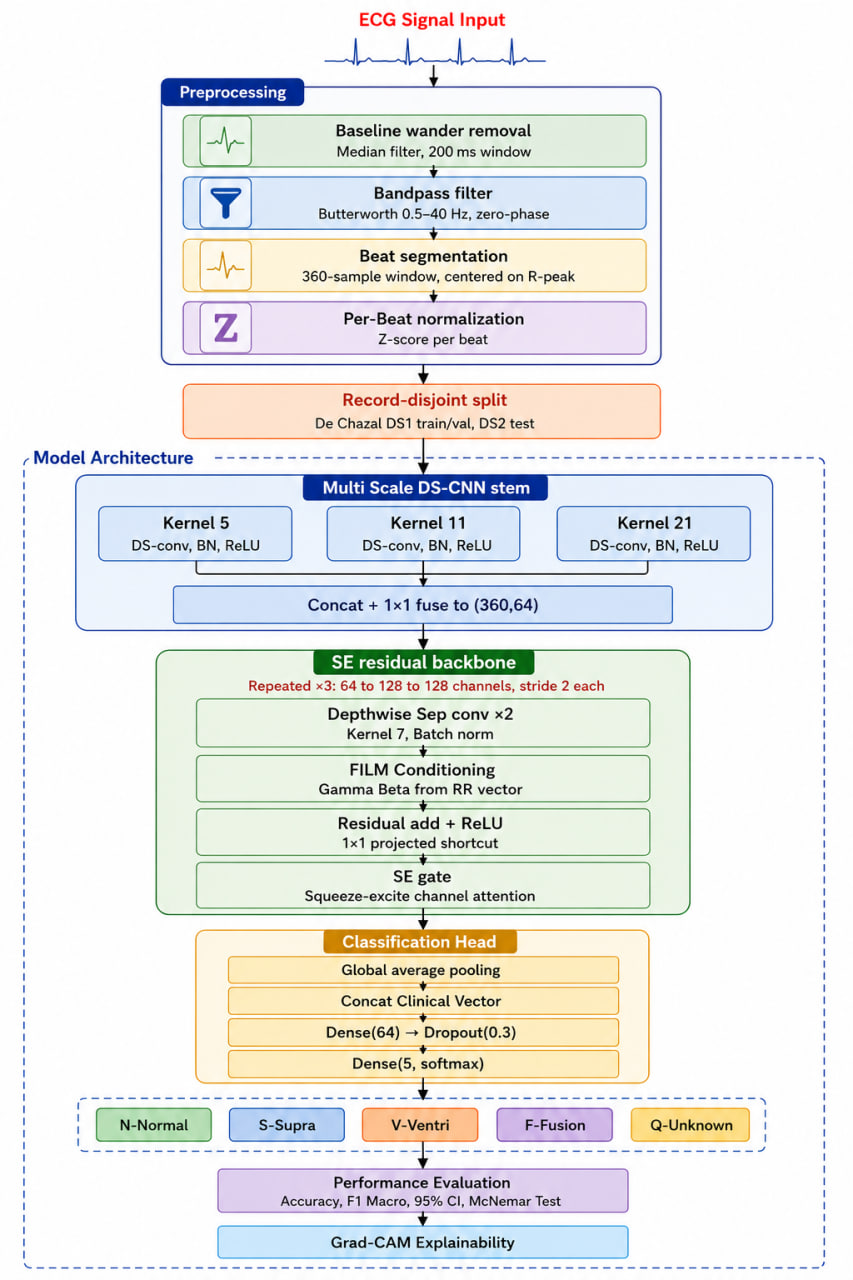
\includegraphics[width=0.95\linewidth]{figures/System_Architecture/msft_net_architecture.png}%
}{%
  \fbox{\parbox[c][2.6in][c]{0.92\linewidth}{\centering\footnotesize
    ADD THE MSFT-NET BLOCK DIAGRAM\\[4pt]
    \texttt{figures/System\_Architecture/}\\
    \texttt{msft\_net\_architecture.png}}}%
}
\caption{Block diagram of the inter-patient MSFT-Net architecture with multi-scale stem, squeeze-and-excitation, and FiLM conditioning}
\label{fig:msft_arch}
\end{figure}


\section{Proposed Methodology}
\label{sec:proposed_methodology}

\subsection{Sampling, labels, and record-disjoint partitioning}

The five AAMI groups were mapped to the MIT-BIH annotation symbols. Paced
records 102, 104, 107, and 217 were excluded from the N/S/V/F analysis;
because this rule filters out most $Q$ beats, beats from these records were
kept when the $Q$-class policy was enabled and excluded otherwise. Results
for $Q$ are therefore interpreted with caution, as they rest on very few
patients.

Records, rather than individual beats, were assigned to partitions to avoid
patient leakage, following the de~Chazal convention of separating the
records used for model development from those used for
testing \cite{dechazal2004}. A validation subset of the development records,
sharing no records with the test set, was reserved for early stopping.
Normal-sinus-rhythm and congestive-heart-failure records used in the
auxiliary analyses were likewise assigned by record identifier. Programmatic
checks ensured that no record appeared in more than one partition and that
all required classes were present in the training and test partitions.

Instead of enforcing a single global beat cap, beats were sampled with
per-record quotas via evenly spaced indices, so that every record
contributed observations and long recordings did not dominate the corpus.
Where possible, rare $S$ and $F$ beats were preserved. Splitting,
resampling, augmenting, scaling, template building, and imbalance correction
were applied only to the training partition.

\subsection{Fusion-beat treatment}

A staged intervention was designed for the fusion class: (i) global-average
pooling in place of attention pooling, (ii) $F$-specific augmentation,
(iii) $F/V$ hard-negative mining, and (iv) auxiliary $F$-vs-$N$ and
$F$-vs-$V$ heads. Each stage was studied in isolation in a dedicated
ablation arm so that its contribution could be measured rather than guessed
at.

\subsection{Microcontroller model}

A separate, single-input CNN was derived for the microcontroller
implementation. The model was quantised to full INT8 with
post-training quantisation using representative calibration beats, checked
against the TensorFlow Lite Micro operator set, and evaluated for accuracy
loss, latency, and memory footprint.


\section{System Workflow}
\label{sec:workflow}

\subsection{Training and imbalance handling}

Models were trained with the Adam optimiser, categorical cross-entropy
loss, a batch size of 64, and up to 50 epochs. Early stopping, learning-rate
decay on plateau, and checkpointing of the best model were all applied using
the validation set. Three class-imbalance strategies were compared: no
correction, a class-weighted loss function, and SMOTE oversampling applied
to the training data only, not the test data \cite{chawla2002smote}. Class
weights were calculated after oversampling and were never combined with
SMOTE. Auxiliary experiments applied conservative class-specific
augmentation, hard-negative mining (for $F$-vs-$V$ and $Q$), and auxiliary
heads (for $F$-vs-$N$, $F$-vs-$V$, and $Q$-vs-rest discrimination).


\section{Performance Evaluation Criteria}
\label{sec:eval_criteria}

\subsection{Primary metrics}

Class-specific sensitivity (Se) and positive predictivity ($+P$), reported
as both gross (pooled-beat) and average (per-record) figures, were the
primary results, as recommended by the ANSI/AAMI EC57 standard
\cite{aami_ec57_2012}. Precision--recall curves, precision at fixed recall,
macro-$F_1$, and accuracy were also reported. The macro-$F_1$ is defined as
the unweighted mean of the per-class $F_1$ scores, where each
$F_1 = 2 \cdot P \cdot R/(P + R)$ with $P$ the precision and $R$ the recall.

\subsection{Statistical analysis}

95\% confidence intervals for proportions were constructed using Wilson's
method \cite{wilson1927}. The 95\% confidence interval for macro-$F_1$ was
estimated with a nonparametric bootstrap using 2,000 resamples. Paired test
predictions were compared with the continuity-corrected McNemar test
\cite{mcnemar1947}, adjusted for multiple comparisons with the Holm
step-down procedure. All tests were two-tailed, and $P < 0.05$ was
considered statistically significant.

\subsection{Robustness and provenance}

Robustness was assessed under additive Gaussian noise (signal-to-noise
ratio from 20~dB down to 0~dB) and under increasing simulated baseline
wander. Source confounding was probed with a logistic-regression
discriminator trained to distinguish normal beats of the MIT-BIH database
from those of the normal-sinus-rhythm database, followed by a re-analysis
of the bandwidth-equalisation experiment.

\subsection{Explainability}

Model explanations were produced with Grad-CAM \cite{selvaraju2017gradcam},
attention weights, and Integrated Gradients \cite{sundararajan2017integrated}.
Faithfulness was assessed with deletion curves, which plot the decrease in
target-class probability after successively masking the most highly
attributed samples against the decrease from random masking.